\subsubsection{Rotation-numbers in the \Glsentrylong{pal} Structures}

Next, we derive rules for the rotation-numbers in the Farey-trees of the \gls{pal} structures.
Note that we don't have two branches in the archetypal model, instead we have four.
This means that the definition \Cref{def:rotation.numbers} does not work for our case.
Instead, we define rotation-tuples.
\Cref{fig:add.prop.rot.num.tree} shows as Farey-tree with rotation-tuples.

\begin{definition}[Rotation Tuples]
	The rotation tuple of a cycle with the symbolic sequence $\phi$ in the archetypal model is defined as the following.
	\begin{align}
		\rho(\phi)
		= \left(\rho_\A(\phi), \rho_\B(\phi), \rho_\C(\phi), \rho_\D(\phi)\right)
		= \left(\dfrac{|\phi|_\A}{|\phi|}, \dfrac{|\phi|_\B}{|\phi|}, \dfrac{|\phi|_\C}{|\phi|}, \dfrac{|\phi|_\D}{|\phi|}\right)
	\end{align}
	Where $|\phi|_\A$ is the number of symbols $\A$ in the sequence.
	Analogous for the symbols $\B$, $\C$, and $\D$.
\end{definition}

\begin{figure}
	\centering
	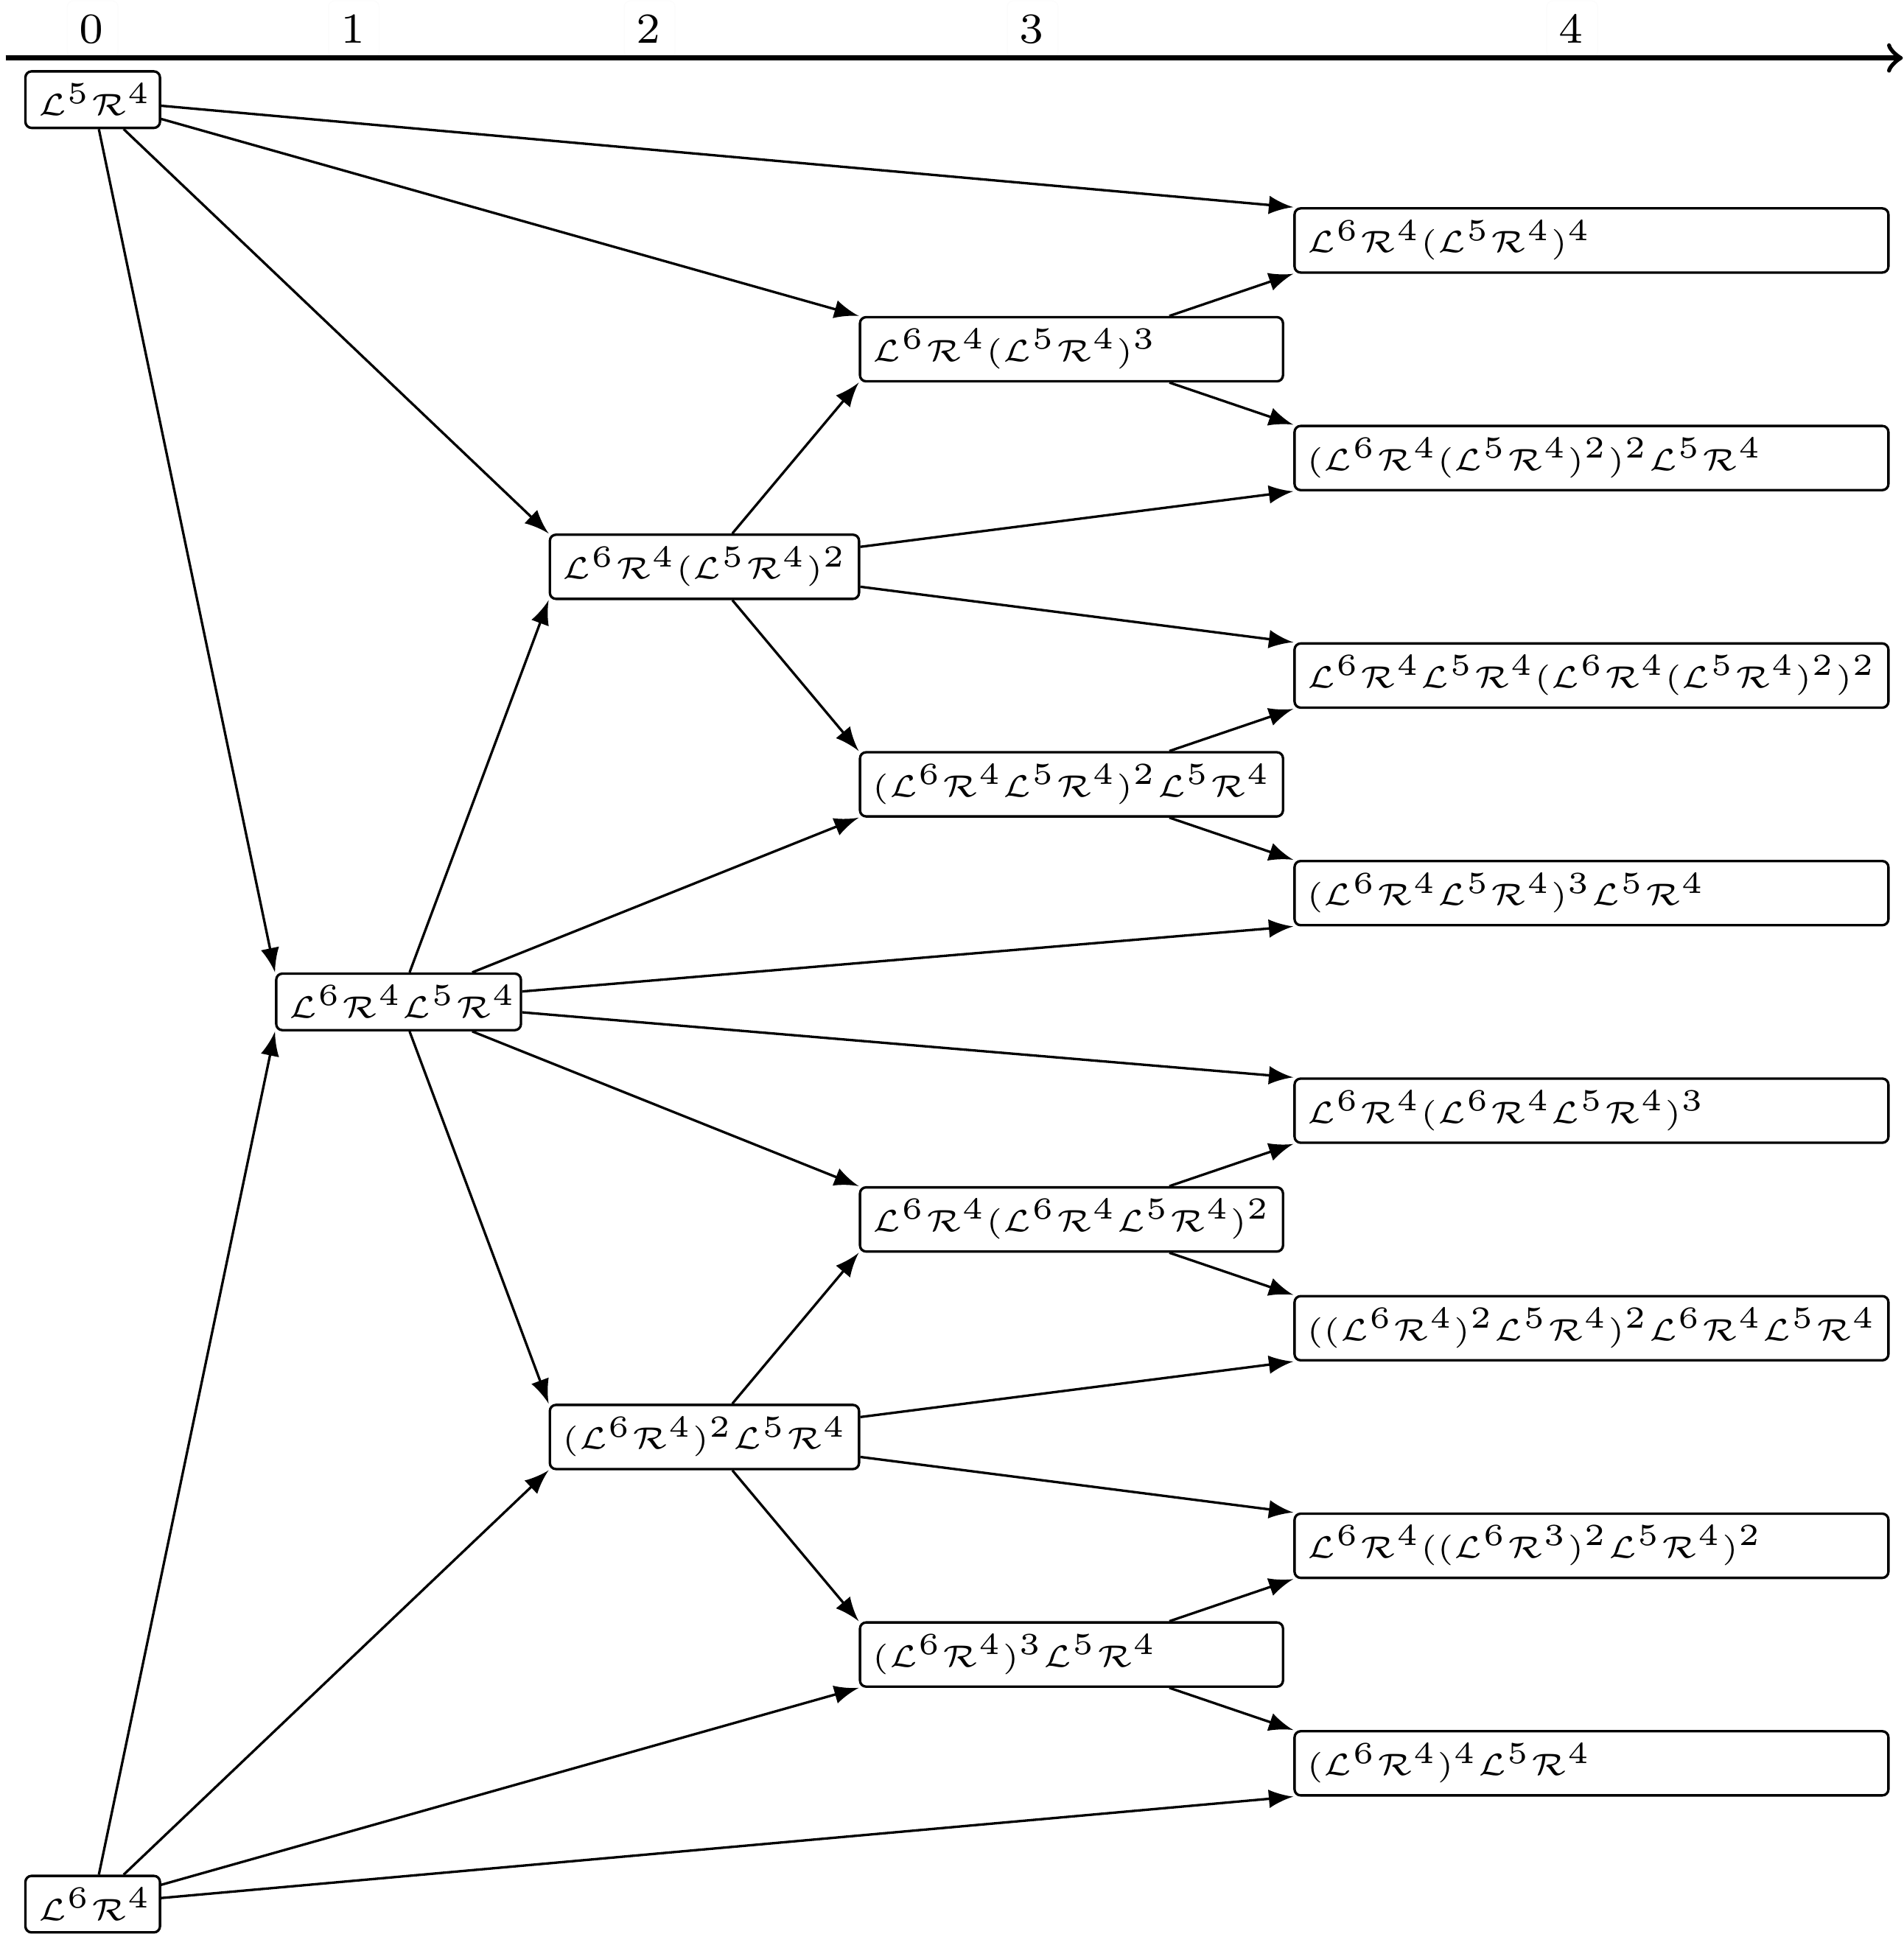
\includegraphics[width=.8 \textwidth]{FareyTrees/Minrep_Adding1_Full_RotNum/adding.png}
	\caption[Farey-tree with rotation tuples of the horizontal \glsentrylong{pal} structure in the archetypal model described in \Cref{sec:add.add.like}]{
		Farey-tree with rotation tuples of the horizontal \glsentrylong{pal} structure in the archetypal model described in \Cref{sec:add.add.like}.
	}
	\label{fig:add.prop.rot.num.tree}
\end{figure}

\begin{theorem}[Rotation Tuples in Child Nodes I]
	The child node of two nodes that are both associated with a single cycle each with the symbolic sequences $\phi$ and $\psi$ is associated with the following period.
	In the following, we call the symbolic sequences of the two twin cycles associated with the child node $\pi^a$ and $\pi^b$.
	\begin{align}
		|\pi^a| = |\pi^b| & = \dfrac{|\phi| + |\psi|}{2} = |\pi|
	\end{align}
	And its associated rotation tuples are:
	\begin{align}
		\rho(\pi^a) = (\rho_\A(\pi^a), \rho_\B(\pi^a), \rho_\C(\pi^a), \rho_\D(\pi^a))
	\end{align}
	and
	\begin{align}
		\rho(\pi^b) = (\rho_\A(\pi^b), \rho_\B(\pi^b), \rho_\C(\pi^b), \rho_\D(\pi^b))
	\end{align}
	Where the elements of each tuple are defined by the following equations.
	\begin{subequations}
		\begin{align}
			\rho_\A(\pi^a) & = \dfrac{\left|\phi_1 \dots \phi_{\frac{n+1}{2}}\right|_\A + \left|\psi_{\frac{m+3}{2}} \dots \psi_m\right|_\A}{|\pi|} \\
			\rho_\B(\pi^a) & = \dfrac{\left|\phi_1 \dots \phi_{\frac{n+1}{2}}\right|_\B + \left|\psi_{\frac{m+3}{2}} \dots \psi_m\right|_\B}{|\pi|} \\
			\rho_\C(\pi^a) & = \dfrac{\left|\phi_1 \dots \phi_{\frac{n-1}{2}}\right|_\C + \left|\psi_{\frac{m+1}{2}} \dots \psi_m\right|_\C}{|\pi|} \\
			\rho_\D(\pi^a) & = \dfrac{\left|\phi_1 \dots \phi_{\frac{n-1}{2}}\right|_\D + \left|\psi_{\frac{m+1}{2}} \dots \psi_m\right|_\D}{|\pi|}
		\end{align}
	\end{subequations}
	and
	\begin{subequations}
		\begin{align}
			\rho_\A(\pi^b) & = \dfrac{\left|\psi_1 \dots \psi_{\frac{m+1}{2}}\right|_\A + \left|\phi_{\frac{n+3}{2}} \dots \phi_n\right|_\A}{|\pi|} \\
			\rho_\B(\pi^b) & = \dfrac{\left|\psi_1 \dots \psi_{\frac{m+1}{2}}\right|_\B + \left|\phi_{\frac{n+3}{2}} \dots \phi_n\right|_\B}{|\pi|} \\
			\rho_\C(\pi^b) & = \dfrac{\left|\psi_1 \dots \psi_{\frac{m-1}{2}}\right|_\C + \left|\phi_{\frac{n+1}{2}} \dots \phi_n\right|_\C}{|\pi|} \\
			\rho_\D(\pi^b) & = \dfrac{\left|\psi_1 \dots \psi_{\frac{m-1}{2}}\right|_\D + \left|\phi_{\frac{n+1}{2}} \dots \phi_n\right|_\D}{|\pi|}
		\end{align}
	\end{subequations}
\end{theorem}

\begin{proof} \phantom{x} \\
	Let $\sigma = \sigma_1\sigma_2 \dots \sigma_i$ with odd $i$, $\varrho = \varrho_1\varrho_2 \dots \varrho_j$ with odd $j$, $T(\sigma) = \phi$, and $T(\varrho) = \psi$.
	The child of both nodes in the halved archetypal model is associated with the symbolic sequence $\sigma\varrho = \sigma_1 \dots \sigma_i \varrho_1 \dots \varrho_j$.
	This manifests as two coexisting cycles in the archetypal model with the symbolic sequences $\pi^a$ and $\pi^b$ following the rules in \Cref{theorem:child.symbolic.1}.

	We start by proving the period of the cycles with symbolic sequences $\pi^a$ and $\pi^b$.
	\begin{align*}
		|\pi^a| & = |T(\sigma\varrho)|                                                                \\
		        & = |T(\sigma_1 \dots \sigma_i \varrho_1 \dots \varrho_j)|                            \\
		        & = |t(\sigma_1\sigma_2) \dots t(\sigma_i\varrho_1) \dots t(\varrho_{j-1}\varrho_j)|  \\
		        & = |\sigma_1\sigma_2 \dots \sigma_i \varrho_1 \dots \varrho_{j-1}\varrho_j|          \\
		        & = |\sigma\varrho| = \frac{|\phi|}{2} + \frac{|\psi|}{2} = \frac{|\phi| + |\psi|}{2}
	\end{align*}
	Note that the last step takes advantage of the fact about the periods of cycles in the archetypal model described in \Cref{theorem:period.pal}.
	The proof for $\pi^b$ is similar and leads to the same result.
	\begin{align*}
		|\pi^b| & = |T(s_2(\sigma\varrho))|                                                                              \\
		        & = |T(\sigma_2 \dots \sigma_i \varrho_1 \dots \varrho_j \sigma_1)|                                      \\
		        & = |t(\sigma_2\sigma_3) \dots t(\sigma_{i-1}\sigma_i) t(\varrho_1\varrho_2) \dots t(\varrho_j\sigma_1)| \\
		        & = |\sigma_2\sigma_3 \dots \sigma_i \varrho_1 \dots \varrho_j \sigma_1|                                 \\
		        & = |\sigma_1\sigma_2 \dots \sigma_i \varrho_1 \dots \varrho_j|                                          \\
		        & = |\sigma\varrho| = \frac{|\phi|}{2} + \frac{|\psi|}{2} = \frac{|\phi| + |\psi|}{2}
	\end{align*}

	This gives us the denominators of all elements of both rotation tuples.
	For the numerators, we have to count the symbols in the symbolic sequences of the cycles associated with each child node.
	We start with $\pi^a$ and the symbol $\A$.
	\begin{align*}
		|\pi^a|_\A & = \left|\phi_1 \dots \phi_{\frac{n-1}{2}} \left[\phi_{\frac{n+1}{2}} \mid \psi_{\frac{m+1}{2}}\right] \psi_{\frac{m+3}{2}} \dots \psi_m\right|_\A                \\
		           & = |\phi_1|_\A + \dots + \left|\left[\phi_{\frac{n+1}{2}} \mid \psi_{\frac{n+1}{2}}\right]\right|_\A + \left|\psi_{\frac{m+3}{2}}\right|_\A + \dots + |\psi_m|_\A \\
		           & = |\phi_1|_\A + \dots + \left|\phi_{\frac{n+1}{2}}\right|_\A + \left|\psi_{\frac{m+3}{2}}\right|_\A + \dots + |\psi_m|_\A                                        \\
		           & = \left|\phi_1 \dots \phi_{\frac{n+1}{2}}\right|_\A + \left|\psi_{\frac{m+3}{2}} \dots \psi_m\right|_\A
	\end{align*}
	We can do the second to last step, since the symbol $\A$ is in the first 2-syllable of $\phi_{\frac{n+1}{2}}$.
	The same is true for the symbol $\B$ and the proof works exactly the same for $|\pi^a|_\B$, so we will omit it here.
	For the symbols $\C$ and $\D$ the last step does not work, instead we have to choose $\psi_{\frac{n+1}{2}}$.
	We demonstrate it for $|\pi^a|_\C$, the proof for $|\pi^a|_\D$ works exactly the same.
	\begin{align*}
		|\pi^a|_\C & = \left|\phi_1 \dots \phi_{\frac{n-1}{2}} \left[\phi_{\frac{n+1}{2}} \mid \psi_{\frac{m+1}{2}}\right] \psi_{\frac{m+3}{2}} \dots \psi_m\right|_\C                \\
		           & = |\phi_1|_\C + \dots + \left|\left[\phi_{\frac{n+1}{2}} \mid \psi_{\frac{n+1}{2}}\right]\right|_\C + \left|\psi_{\frac{m+3}{2}}\right|_\C + \dots + |\psi_m|_\C \\
		           & = |\phi_1|_\C + \dots + \left|\psi_{\frac{n+1}{2}}\right|_\C + \left|\psi_{\frac{m+3}{2}}\right|_\C + \dots + |\psi_m|_\C                                        \\
		           & = \left|\phi_1 \dots \psi_{\frac{n+1}{2}}\right|_\C + \left|\psi_{\frac{m+3}{2}} \dots \psi_m\right|_\C
	\end{align*}

	Now we will take a look at the numerators of the elements in the rotation tuple of $\pi^b$.
	We start with the symbol $\A$.
	\begin{align*}
		|\pi^b|_\A & = \left|\phi_{\frac{n+3}{2}} \dots \phi_n \psi_1 \dots \psi_{\frac{m-1}{2}} \left[\psi_{\frac{m+1}{2}} \mid \phi_{\frac{n+1}{2}}\right]\right|_\A                                                       \\
		           & = \left|\phi_{\frac{n+3}{2}}\right|_\A + \dots + |\phi_n|_\A + |\psi_1|_\A + \dots + \left|\psi_{\frac{m-1}{2}}\right|_\A + \left|\left[\psi_{\frac{m+1}{2}} \mid \phi_{\frac{n+1}{2}}\right]\right|_\A \\
		           & = \left|\phi_{\frac{n+3}{2}}\right|_\A + \dots + |\phi_n|_\A + |\psi_1|_\A + \dots + \left|\psi_{\frac{m-1}{2}}\right|_\A + \left|\psi_{\frac{m+1}{2}}\right|_\A                                        \\
		           & = \left|\phi_{\frac{n+3}{2}} \dots \phi_n\right|_\A + \left|\psi_1 \dots \psi_{\frac{m-1}{2}}\right|_\A + \left|\psi_{\frac{m+1}{2}}\right|_\A
	\end{align*}
	Again, we can do the second to last step, since the symbol $\A$ is in the first 2-syllable of $\psi_{\frac{n+1}{2}}$.
	The same is true for the symbol $\B$ and the proof works exactly the same for $|\pi^b|_\B$.
	We will omit it here.
	For the symbols $\C$ and $\D$ the last step does not work, instead we have to choose $\phi_{\frac{n+1}{2}}$.
	We demonstrate it for $|\pi^b|_\C$, the proof for $|\pi^b|_\D$ works exactly the same.
	\begin{align*}
		|\pi^b|_\C & = \left|\phi_{\frac{n+3}{2}} \dots \phi_n \psi_1 \dots \psi_{\frac{m-1}{2}} \left[\psi_{\frac{m+1}{2}} \mid \phi_{\frac{n+1}{2}}\right]\right|_\C                                                       \\
		           & = \left|\phi_{\frac{n+3}{2}}\right|_\C + \dots + |\phi_n|_\A + |\psi_1|_\C + \dots + \left|\psi_{\frac{m-1}{2}}\right|_\C + \left|\left[\psi_{\frac{m+1}{2}} \mid \phi_{\frac{n+1}{2}}\right]\right|_\C \\
		           & = \left|\phi_{\frac{n+3}{2}}\right|_\C + \dots + |\phi_n|_\C + |\psi_1|_\C + \dots + \left|\psi_{\frac{m-1}{2}}\right|_\C + \left|\psi_{\frac{m+1}{2}}\right|_\C                                        \\
		           & = \left|\phi_{\frac{n+3}{2}} \dots \phi_n\right|_\C + \left|\psi_1 \dots \psi_{\frac{m-1}{2}} \psi_{\frac{m+1}{2}}\right|_\C
	\end{align*}
	\hfill $\blacksquare$
\end{proof}

\begin{theorem}[Rotation Tuples in Child Nodes II]
	The child node of a node that is associated with a single cycle $\phi$ and a node that is associated with two coexisting cycles with the symbolic sequences $\psi^a$ and $\psi^b$ is associated with the following rotation tuple.
	We use element-wise Farey-addition here, since it is the same for each symbol.
	\begin{align}
		\rho(\pi) = \rho(\phi) \oplus \rho(\psi^a) \oplus \rho(\psi^b)
	\end{align}
\end{theorem}

\begin{proof} \phantom{x} \\
	We prove this again in two parts.
	First, we prove that the denominator of each element of the rotation tuples add up.
	\begin{align*}
		|\pi| & = \left|
		\phi_1 \dots \phi_{\frac{n-1}{2}} \left[\phi_{\frac{n+1}{2}} \mid \psi^b_m\right]
		\psi^b_1 \dots \psi^b_{m-1} \left[\psi^b_m \mid \phi_{\frac{n+1}{2}}\right]
		\phi_{\frac{n+3}{2}} \dots \phi_n \psi^a
		\right|                                                       \\
		      & = \left|
		\phi_1 \dots \phi_{\frac{n-1}{2}} \left[\phi_{\frac{n+1}{2}} \mid \phi_{\frac{n+1}{2}}\right]
		\phi_{\frac{n+3}{2}} \dots \phi_n
		\psi^b_1 \dots \psi^b_{m-1} \left[\psi^b_m \mid \psi^b_m\right]
		\psi^a
		\right|                                                       \\
		      & = |\phi \psi^b \psi^a| = |\phi| + |\psi^a| + |\psi^b|
	\end{align*}
	Note that the first step is achieved by simply reordering some 4-syllables and two 2-syllables in the symbolic sequences.
	This does not change the period.
	It does also not change the number of symbols, since we only swapped the second 2-syllable of $\left[\phi_{\frac{n+1}{2}} \mid \psi^b_m\right]$ and $\left[\psi^b_m \mid \phi_{\frac{n+1}{2}}\right]$.
	Therefore, the proof for works the same for the number of any symbol.
	We will demonstrate this for symbol $\A$.
	\begin{align*}
		|\pi|_\A & = \left|
		\phi_1 \dots \phi_{\frac{n-1}{2}} \left[\phi_{\frac{n+1}{2}} \mid \psi^b_m\right]
		\psi^b_1 \dots \psi^b_{m-1} \left[\psi^b_m \mid \phi_{\frac{n+1}{2}}\right]
		\phi_{\frac{n+3}{2}} \dots \phi_n \psi^a
		\right|_\A                                                                   \\
		         & = \left|
		\phi_1 \dots \phi_{\frac{n-1}{2}} \left[\phi_{\frac{n+1}{2}} \mid \phi_{\frac{n+1}{2}}\right]
		\phi_{\frac{n+3}{2}} \dots \phi_n
		\psi^b_1 \dots \psi^b_{m-1} \left[\psi^b_m \mid \psi^b_m\right]
		\psi^a
		\right|_\A                                                                   \\
		         & = |\phi \psi^b \psi^a|_\A = |\phi|_\A + |\psi^a|_\A + |\psi^b|_\A
	\end{align*}
	Therefore, the numerators of each element in the rotation tuples add up too.

	One might criticize that we only proved it for the case where the left parent node is associated with a single cycle.
	In that case
	\begin{align*}
		\pi = \phi_1 \dots \phi_{\frac{n-1}{2}} \left[\phi_{\frac{n+1}{2}} \mid \psi^b_m\right] \psi^b_1 \dots \psi^b_{m-1} \left[\psi^b_m \mid \phi_{\frac{n+1}{2}}\right] \phi_{\frac{n+3}{2}} \dots \phi_n \psi^a
	\end{align*}
	If the right parent node is associated with a single cycle, then
	\begin{align*}
		\pi = \psi^a \phi_1 \dots \phi_{\frac{n-1}{2}} \left[\phi_{\frac{n+1}{2}} \mid \psi^b_m\right] \psi^b_1 \dots \psi^b_{m-1} \left[\psi^b_m \mid \phi_{\frac{n+1}{2}}\right] \phi_{\frac{n+3}{2}} \dots \phi_n
	\end{align*}
	The only difference in both cases is that the symbols of $\psi^a$ are at the end of the symbolic sequence in the first case and at the beginning of the symbolic sequence in the second case.
	Since reordering of 4-syllables does not change the period nor the number of individual symbols, this proof works for both cases.

	\hfill $\blacksquare$
\end{proof}

As mentioned before, the next case does not appear in the \gls{pal} structures we investigate.
But we will include it here again for completeness.

\begin{theorem}[Rotation Tuples in Child Nodes III]
	The child node of two nodes that are both associated with two coexisting cycles each with symbolic sequences $\phi^a, \phi^b, \psi^a,$ and $\psi^b$ is associated with two coexisting cycles.
	Their rotation tuples are the defined by the following equations.
	Note that we use element-wise Farey-addition here again.
	\begin{align}
		\rho(\pi^a) & = \rho(\phi^a) \oplus \rho(\psi^a)
	\end{align}
	and
	\begin{align}
		\rho(\pi^b) & = \rho(\phi^b) \oplus \rho(\psi^b)
	\end{align}
\end{theorem}

\begin{proof} \phantom{x} \\
	We start with the cycle with symbolic sequence $\pi^a$.
	Again, we first prove that the denominators, i.e. the periods, add up.
	\begin{align*}
		|\pi^a| = |\phi^a\psi^a| = |\phi^a| + |\psi^a|
	\end{align*}
	This is straightforward and can be done for each symbol exactly like this.
	We will demonstrate it for the symbol $\A$.
	\begin{align*}
		|\pi^a|_\A = |\phi^a\psi^a|_\A = |\phi^a|_\A + |\psi^a|_\A
	\end{align*}
	Therefore, the numerators also add up.

	Now we prove the same thing for the cycle with symbolic sequence $\pi^b$.
	\begin{align*}
		|\pi^b| & = \left|\phi^b_1 \dots \phi^b_{n-1} \left[\phi^b_n \mid \psi^b_m\right] \psi^b_1 \dots \psi^b_{m-1} \left[\psi^b_m \mid \phi^b_n\right]\right| \\
		        & = \left|\phi^b_1 \dots \phi^b_{n-1} \left[\phi^b_n \mid \phi^b_n\right] \psi^b_1 \dots \psi^b_{m-1} \left[\psi^b_m \mid \psi^b_m\right]\right| \\
		        & = |\phi^b \psi^b| = |\phi^b| + |\psi^b|
	\end{align*}
	Here we simply swapped the second 2-syllables of $\left[\phi^b_n \mid \psi^b_m\right]$ and $\left[\psi^b_m \mid \phi^b_n\right]$.
	This does not change the period.
	It also does not change the number of any symbol.
	Therefore, we can use the same proof for any symbol and show that the numerators also add up.
	We demonstrate it for the symbol $\A$ in the following.
	\begin{align*}
		|\pi^b|_\A & = \left|\phi^b_1 \dots \phi^b_{n-1} \left[\phi^b_n \mid \psi^b_m\right] \psi^b_1 \dots \psi^b_{m-1} \left[\psi^b_m \mid \phi^b_n\right]\right|_\A \\
		           & = \left|\phi^b_1 \dots \phi^b_{n-1} \left[\phi^b_n \mid \phi^b_n\right] \psi^b_1 \dots \psi^b_{m-1} \left[\psi^b_m \mid \psi^b_m\right]\right|_\A \\
		           & = |\phi^b \psi^b|_\A = |\phi^b|_\A + |\psi^b|_\A
	\end{align*}
	\hfill $\blacksquare$
\end{proof}

In the usual case with two symbols, the rotation numbers are monotone.
In our case we have rotation tuples instead of numbers, and we will consider the monotonicity of the single elements.
Also, we sometimes have coexistence of two cycles.
We will consider the rotation tuples of each of the coexisting twin cycles independently.
The monotonicity does not hold up for our case, unfortunately.
We can see a counter example in \Cref{fig:add.prop.rot.num.tree}.
Let's consider the rotation numbers for the symbol $\A$ which are the first element in each rotation tuple.
The right starting node, the upper node of level 0, is associated with the rotation number $\frac{5}{18}$ for the symbol $\A$.
And the left starting node is associated with the rotation number $\frac{6}{20}$ for the symbol $\A$.
And $\frac{6}{20} > \frac{5}{18}$, so each rotation number for the symbol $\A$ of the coexisting cycles associated with the child node should be in-between those two numbers.
But the rotation numbers for the symbol $\A$ in the child node are $\frac{6}{19} > \frac{6}{20}$ and $\frac{5}{19} < \frac{5}{18}$.
If we instead consider the element-wise Farey-sum of both rotation tuples in the case of coexisting cycles, the monotonicity holds.

\begin{theorem}[Monotonicity of Rotation Tuples in \gls{pal} Structures]
	\label{theorem:rotation.monotonicity}
	Let the rotation tuple of the left starting node be element-wise smaller than the rotation tuple of the right starting node w.l.o.g.
	Then the rotation tuple of a node that is associated with a cycle $\phi$ is element-wise smaller than the rotation tuple of a node that is associated with a cycle $\psi$,
	if the node associated with $\phi$ is \hl{to} left of the node associated with $\psi$ in the Farey-tree.
\end{theorem}

\begin{proof} \phantom{x} \\
	This is a proof by induction, and it will rely heavily on the following fact.
	If $\frac{a_1}{b_1} < \frac{a_2}{b_2}$, then
	\begin{align}
		\frac{a_1}{b_1} < \frac{a_1}{b_1} \oplus \frac{a_2}{b_2} < \frac{a_2}{b_2}
	\end{align}

	We consider the structure of the Farey-tree like in the proof for \Cref{theorem:no.parent.coex}.
	First, we write down the starting nodes.
	Here, the only content is the rotation tuples and the left starting node is element-wise smaller than the right starting node w.l.o.g.
	Note that for coexisting twin cycles $\pi^a$ and $\pi^b$, we consider the element-wise Farey-sum of their rotation tuples $\rho(\pi) = \rho(\pi^a) \oplus \rho(\pi^b)$.
	For each iteration we combine each pair of rotation tuples in the list and insert the result in the middle of each pair.
	We again reformulate the statement of \Cref{theorem:rotation.monotonicity} to a statement about the lists at each iteration.

	In all lists, the node $\rho(\phi)$ will be element-wise smaller than the next node $\rho(\psi)$.
	This implies global monotonicity at each iteration for the lists.
	And therefore also global monotonicity in the Farey-tree across all levels.

	\begin{itemize}
		\item[n = 0] The left starting node is element-wise smaller than the right starting node by construction.
		\item[n + 1] We assume that the above statement is true for the current list of $2^n$.
			And we proof that for each neighboring nodes $\{\dots ,\rho(\phi), \rho(\psi), ...\}$ the values of their child node $\rho(\pi)$ is in-between the values of its two parent nodes.
			\begin{align*}
				\rho(\phi) < \rho(\pi) < \rho(\psi)
			\end{align*}
			We need to consider four cases.
			First, let's assume that the node associated with $\rho(\phi)$ is associated with a single cycle when considering the Farey-tree with symbolic sequences and the node associated with $\rho(\psi)$ is also associated with a single cycle.
			Then for symbol $\A$
			\begin{align*}
				\rho_\A(\pi) & = \rho_\A(\pi^a) \oplus \rho_\A(\pi^b)                                                                       \\
				             & =
				\dfrac{\left|\phi_1 \dots \phi_{\frac{n+1}{2}}\right|_\A + \left|\psi_{\frac{m+3}{2}} \dots \psi_m\right|_\A}{|\pi|}
				\oplus \dfrac{\left|\psi_1 \dots \psi_{\frac{m+1}{2}}\right|_\A + \left|\phi_{\frac{n+3}{2}} \dots \phi_n\right|_\A}{|\pi|} \\
				             & =
				\dfrac
				{\left|\phi_1 \dots \phi_{\frac{n+1}{2}}\right|_\A + \left|\psi_{\frac{m+3}{2}} \dots \psi_m\right|_\A + \left|\psi_1 \dots \psi_{\frac{m+1}{2}}\right|_\A + \left|\phi_{\frac{n+3}{2}} \dots \phi_n\right|_\A}
				{2 \cdot |\pi|}                                                                                                             \\
				             & =
				\dfrac
				{\left|\phi_1 \dots \phi_{\frac{n+1}{2}} \psi_{\frac{m+3}{2}} \dots \psi_m \psi_1 \dots \psi_{\frac{m+1}{2}} \phi_{\frac{n+3}{2}} \dots \phi_n\right|_\A}
				{2 \cdot \frac{|\phi| + |\psi|}{2}}                                                                                         \\
				             & =
				\dfrac
				{\left|\phi_1 \dots \phi_{\frac{n+1}{2}} \phi_{\frac{n+3}{2}} \dots \phi_n \psi_1 \dots \psi_{\frac{m+1}{2}} \psi_{\frac{m+3}{2}} \dots \psi_m\right|_\A}
				{|\phi| + |\psi|}                                                                                                           \\
				             &
				= \dfrac{|\phi\psi|_\A}{|\phi| + |\psi|}
				= \dfrac{|\phi|_\A + |\psi|_\A}{|\phi| + |\psi|}
				= \rho_\A(\phi) \oplus \rho_\A(\psi)
			\end{align*}
			And since $\rho_\A(\phi) < \rho_\A(\psi) \implies \rho_\A(\phi) < \rho_\A(\phi) \oplus \rho_\A(\psi) < \rho_\A(\psi)$,
			it also implies that $\rho_\A(\phi) < \rho_\A(\pi) =  \rho_\A(\pi^a) \oplus \rho_\A(\pi^h) < \rho_\A(\psi)$.

			This works exactly the same for the symbol $\B$, and we will omit it here.
			For the symbols $\C$ and $\D$ it is slightly different.
			We will demonstrate it for the symbol $\C$ in the following.
			\begin{align*}
				\rho_\C(\pi) & = \rho_\C(\pi^a) \oplus \rho_\C(\pi^b)                                                                       \\
				             & =
				\dfrac{\left|\phi_1 \dots \phi_{\frac{n-1}{2}}\right|_\C + \left|\psi_{\frac{m+1}{2}} \dots \psi_m\right|_\C}{|\pi|}
				\oplus \dfrac{\left|\psi_1 \dots \psi_{\frac{m-1}{2}}\right|_\C + \left|\phi_{\frac{n+1}{2}} \dots \phi_n\right|_\C}{|\pi|} \\
				             & =
				\dfrac
				{\left|\phi_1 \dots \phi_{\frac{n-1}{2}}\right|_\C + \left|\psi_{\frac{m+1}{2}} \dots \psi_m\right|_\C + \left|\psi_1 \dots \psi_{\frac{m-1}{2}}\right|_\C + \left|\phi_{\frac{n+1}{2}} \dots \phi_n\right|_\C}
				{2 \cdot |\pi|}                                                                                                             \\
				             & =
				\dfrac
				{\left|\phi_1 \dots \phi_{\frac{n-1}{2}} \psi_{\frac{m+1}{2}} \dots \psi_m \psi_1 \dots \psi_{\frac{m-1}{2}} \phi_{\frac{n+1}{2}} \dots \phi_n\right|_\C}
				{2 \cdot \frac{|\phi| + |\psi|}{2}}                                                                                         \\
				             & =
				\dfrac
				{\left|\phi_1 \dots \phi_{\frac{n-1}{2}} \phi_{\frac{n+1}{2}} \dots \phi_n \psi_1 \dots \psi_{\frac{m-1}{2}} \psi_{\frac{m+1}{2}} \dots \psi_m\right|_\C}
				{|\phi| + |\psi|}                                                                                                           \\
				             &
				= \dfrac{|\phi\psi|_\C}{|\phi| + |\psi|}
				= \dfrac{|\phi|_\C + |\psi|_\C}{|\phi| + |\psi|}
				= \rho_\A(\phi) \oplus \rho_\C(\psi)
			\end{align*}
			And since $\rho_\C(\phi) < \rho_\C(\psi) \implies \rho_\C(\phi) < \rho_\C(\phi) \oplus \rho_\C(\psi) < \rho_\C(\psi)$,
			it also implies that $\rho_\C(\phi) < \rho_\C(\pi) =  \rho_\C(\pi^a) \oplus \rho_\C(\pi^h) < \rho_\C(\psi)$.

			Next, let's consider the case where the node associated with $\rho(\phi)$ is associated with a single cycle when considering the Farey-tree with symbolic sequences and the node associated with $\rho(\psi) = \rho(\psi^a) \oplus \rho(\psi^b)$ is also associated with two coexisting cycles.
			Here, we can use the element-wise Farey-sum and prove it simultaneously for all symbols.
			\begin{align*}
				\rho(\pi) & = \rho(\phi) \oplus \rho(\psi^a) \oplus \rho(\psi^b) \\
				          & = \rho(\phi) \oplus \rho(\psi)
			\end{align*}
			Since $\rho(\phi) < \rho(\psi) \implies \rho(\phi) < \rho(\phi) \oplus \rho(\psi) < \rho(\psi)$, it also implies that $\rho(\phi) < \rho(\pi) = \rho(\phi) \oplus \rho(\psi) < \rho(\psi)$.

			The proof works similar for the third case, where the node associated with $\rho(\phi) = \rho(\phi^a) \oplus \rho(\phi^b)$ is also associated with two coexisting cycles and the node associated with $\rho(\psi)$ is associated with a single cycle.
			\begin{align*}
				\rho(\pi) & = \rho(\phi^a) \oplus \rho(\phi^b) \oplus \rho(\psi) \\
				          & = \rho(\phi) \oplus \rho(\psi)
			\end{align*}
			Since $\rho(\phi) < \rho(\psi) \implies \rho(\phi) < \rho(\phi) \oplus \rho(\psi) < \rho(\psi)$, it also implies that $ \rho(\phi) < \rho(\pi) = \rho(\phi) \oplus \rho(\psi) < \rho(\psi)$.

			The last case does not occur in the \gls{pal} structures that we are investigating, but we will include a proof for this case also.
			Both the left node that is associated with $\rho(\phi) = \rho(\phi^a) \oplus \rho(\phi^b)$ and the right node that is associated with $\rho(\psi) = \rho(\psi^a) \oplus \rho(\psi^b)$ are associated with two coexisting cycles.
			Again we can use element-wise Farey-addition.
			\begin{align*}
				\rho(\pi) & = \rho(\pi^a) \oplus \rho(\pi^b)                                                                     \\
				          & = \left(\rho(\phi^a) \oplus \rho(\psi^a)\right) \oplus \left(\rho(\phi^b) \oplus \rho(\psi^b)\right) \\
				          & = \rho(\phi^a) \oplus \rho(\psi^a) \oplus \rho(\phi^b) \oplus \rho(\psi^b)                           \\
				          & = \rho(\phi^a) \oplus \rho(\phi^a) \oplus \rho(\psi^a) \oplus \rho(\psi^b)                           \\
				          & = \rho(\phi) \oplus \rho(\psi)                                                                       \\
			\end{align*}
			And $\rho(\phi) < \rho(\psi) \implies \rho(\phi) < \rho(\pi) = \rho(\phi) \oplus \rho(\psi) < \rho(\psi)$.
	\end{itemize}
	\hfill $\blacksquare$
\end{proof}

This concludes the derived properties and rules for the \gls{pal} structures in the archetypal model.
